\documentclass[10pt,twocolumn,letterpaper]{article}

\usepackage{cvpr}
\usepackage{times}
\usepackage{epsfig}
\usepackage{graphicx}
\usepackage{amsmath}
\usepackage{amssymb}

% Include other packages here, before hyperref.

% If you comment hyperref and then uncomment it, you should delete
% egpaper.aux before re-running latex.  (Or just hit 'q' on the first latex
% run, let it finish, and you should be clear).
\usepackage[breaklinks=true,bookmarks=false]{hyperref}

\cvprfinalcopy % *** Uncomment this line for the final submission

\def\cvprPaperID{****} % *** Enter the CVPR Paper ID here
\def\httilde{\mbox{\tt\raisebox{-.5ex}{\symbol{126}}}}

% Pages are numbered in submission mode, and unnumbered in camera-ready
%\ifcvprfinal\pagestyle{empty}\fi
\setcounter{page}{1}
\begin{document}

%%%%%%%%% TITLE
\title{Music exploration using machine learning }

\author{Jibin Rajan Varghese\\
Texas A\&M University\\
400 Bizzell St, College Station, TX 77843\\
{\tt\small jibin@tamu.edu}
% For a paper whose authors are all at the same institution,
% omit the following lines up until the closing ``}''.
% Additional authors and addresses can be added with ``\and'',
% just like the second author.
% To save space, use either the email address or home page, not both
\and
Mohammed Habibullah Baig\\
Texas A\&M University\\
400 Bizzell St, College Station, TX 77843\\
{\tt\small habib\_baig.tamu@tamu.edu}
}

\maketitle
%\thispagestyle{empty}

%%%%%%%%% ABSTRACT
\begin{abstract}
Music is complex and varies widely in beats, frequencies and structure. This experiment uses the spectrogram of common songs to organize thousands of everyday tracks. We plan to use neural networks to train a classifier to segregate neighboring songs with similar features from the spectrogram and audio meta-data. Finally using dimensionality reduction techniques, the computer places similar songs features closer together on a visually interactive song-map. This, in our research so far, is the first attempt at providing a visual and interactive map of songs that users can use in order to explore the world of music, discover and listen to songs of their preference.
\end{abstract}

%%%%%%%%% BODY TEXT


\section{Introduction}
In recent years, as digital media is evolving rapidly, the choice of people's entertainment is changing greatly. Nowadays, listening to music has become very convenient and cheaper than before, hence new music platforms and websites are emerging rapidly, for example, Spotify, Pandora, Douban FM and so on. Many of these companies already are starting to use machine learning approaches to classify music, and hence research on music recommendation system is catching the attention of a lot of researchers in this field. \\

With people being absorbed in music every day, a visual way to interact and recommend suitable music would greatly enhance user experience with users getting an idea where to look for and discover similar songs of their liking, which currently is a manner of interaction that no current music recommendation system is able to provide.\\ 

To recommend suitable song efficiently, music genres must be identified/predicted with good accuracy. Genres can be thought of as descriptive keywords that convey high-level information about music (Pop, rock, Country, ...). Since songs are too large to be encoded bitwise into a large feature set and processed directly for dimensionality reduction, we need a way to reduce the size of the feature set into a manageable and yet distinguishing subset, which we can generate using neural network and/or deep learning approaches. Finally we perform dimensionality reduction techniques on the reduced feature vectors in order to depict the multi-dimensional song features into 2D or 3D map of songs. Then the user can explore this map in order to discover similar songs of their taste in the neighborhood of songs they already like, or choose to explore songs in a previously unexplored area in order to discover other types of music.

 \begin{figure}
 	\begin{center}
 		\fbox{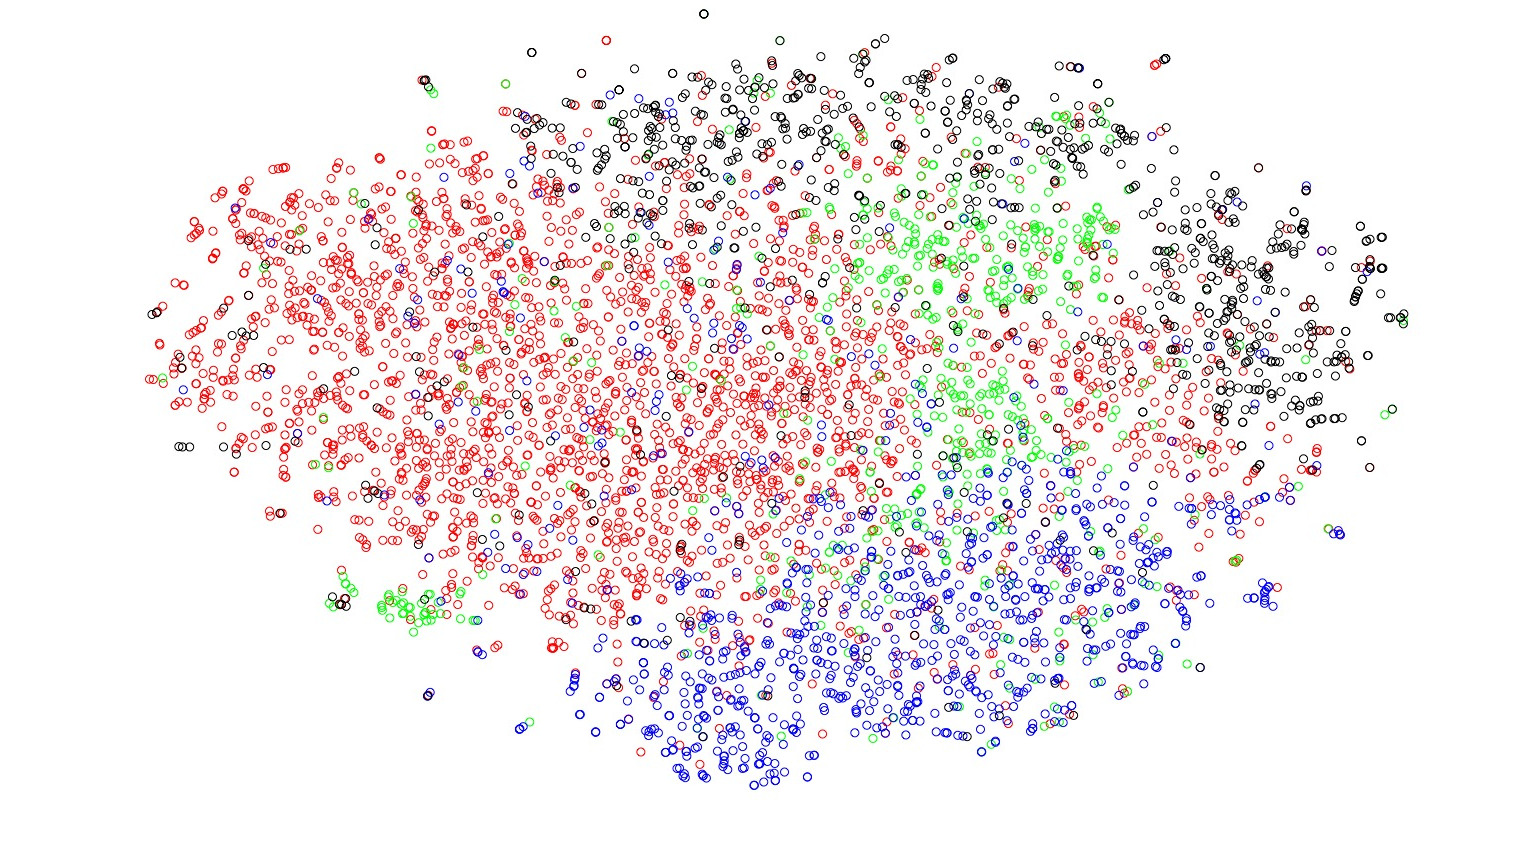
\includegraphics[width=0.8\linewidth]{worldOfMusic.jpg}}	
 	\end{center}
 	\caption{Example of the map of songs we plan to generate. Similar songs will cluster together based on various feature similarities}
 	%\label{fig:long}
 	%\label{fig:onecol}
 \end{figure}

\section {Background}

We need acoustic information about the music to extract the relevant features. Multi-resolution spectrograms can be used to extract suitable features from the audio signal on different time scales \cite{dieleman2013multiscale}.  Paper \cite{li2003comparative} uses three feature sets for representing timbral texture, rhythmic content and pitch content to predict the genres correctly. These features reflected very high information about the music genre as they verified it by training statistical pattern recognition classifiers using real-world audio collections. Additionally, Daubechies wavelet coefficient histograms (DWCHs) \cite{li2003comparative} can also be used, which captures the local and global information of music signals simultaneously by computing wavelet coefficient histograms. . \\

For genre prediction and recommendation the systems currently in use are, \cite{celma2005foafing} which uses the Friend of a Friend (FOAF) and Rich Site Summary (RSS) vocabularies for recommending music to a user, depending on his musical tastes. The other approach in \cite{van2013deep} uses a latent factor model for recommendation, and predict the latent factors from music audio using deep neural net and evaluate the predictions on the Million Song Dataset\cite{bertin2011million}. It was observed that the predicted latent factors gives sensible recommendations, despite the fact that there is a large semantic gap between the characteristics of a song that affect user preference and the corresponding audio signal. One other way would be to have a context-aware recommendation system. Paper \cite{park2006context} exploits the fuzzy system, Bayesian networks and the utility theory in order to recommend appropriate music with respect to the context. \\

Finally, for clustering similar song together and visualizing them, we can use the dimensionality reduction techniques e.g. PCA, LDA. A better approach i.e. t-SNE(t distributed Stochastic Neighbor Embedding ) is suggested in \cite{maaten2008visualizing}. 


\section{Methodology}

We have broken down the main task of music exploration into discrete steps that we will take in order to acomplish the goal of developing a visual way to interact with music. 

\subsection{Song Feature Extraction and Classification}

The first step towards generating the map of songs is to extract meaningful features out of them. These would be features like song genre, beats, timbre, language, artists etc. The raw data of the song and its meta-data would be fed into a neural network and trained using classification labels available. In order to do this we are planning to use a convolutional neural network  or recurrent neural network in order to classify the songs into genres. We can then look for interesting patterns in the outputs of the penultimate layers. This approach has already been tried out in neuroscience and vision \cite{rohit2011convolutional} and we believe using the flattened features of the penultimate layers of neural networks in music will also provide us with a reduced feature set that can be fed into our dimensionality reduction later on.\\

Using the right features are very important to identify genres \cite{zheng2017music} or in our case the right feature vectors of the songs. Here we need to balance out the specificity, ie. response to particular type of song and the generality, ie. the amount of spread of feature vectors when the songs are fed into the system, so that we get a decent but relevant spread in our final song-map. If the outputs of the song classifier are too specific, the final dimensionality reduction will have a lot of data points clustered close together and there will not be sufficient scatter in the data-points in the visualization. On the other hand data that is poorly classified will have a lot of intermixed points which will lead to poor relevance of one song to other.\\

 Thus the aim of the project is not to exceed the performance metric of the existing classification systems, but to tune the results of the neural networks to generate an appropriate set of feature vectors, which upon being fed into the dimensionality reduction system provides us with a map of music which will be relevant to the user.

\subsection{Visualization}

There are multiple methods to perform dimensionality reduction. Principal Component Analysis \cite{wold1987principal} and Linear Discriminant Analysis \cite{izenman2013linear} are two commonly used methods to reduce multidimensional features into two or three dimensions. We are also exploring the use of a technique called t-SNE \cite{maaten2008visualizing} in order to develop the music map. It is a variation of SNE that is much easier to optimize, and produces significantly better visualizations by reducing the tendency to crowd points together in the center of the map. This technique very efficiently visualizes non-parametric high-dimensional data \cite{van2012self} . A summary of some of the most popular dimensionality reduction techniques are given in \cite{bunte2012general}.

\subsection{User Interface}
Finally we aim to use the music map generated by the visualization into a system that allows the user to click and play the songs in the area selected, or let the system recommend and play songs in the nearby area using a random selection that travels from one adjacent song node to the next in the music map. The development of these advanced features in the UI is secondary to the project, as the main challenge would be to develop a relevant mapping of songs.

\section{Datasets}

There are millions of songs in the world to chose from and add to our system. With an impartial feature classifier, we hope to get better and better at mapping songs to the point were any new song released can be added to the system and it will put the song into the right spot on our map. However, given the limitations of time and computing power, we plan to start with smaller song sets and learn the features on smaller subsets of music. Incrementally, we intend to work on the following datasets :

\begin{enumerate}
	\item Manually curated set of around 50-100 songs, which will be basis for the initial training of the classifier.
	\item GTZAN Genre Collection : 	This dataset was used for the well known paper in genre classification \cite{tzanetakis2002musical}. The dataset consists of 1000 audio tracks each 30 seconds long. It contains 10 genres, each represented by 100 tracks. 
	\item The Million Song Dataset \cite{bertin2011million}: This is a freely-available collection of audio features and meta-data for a million contemporary popular music tracks. This is our largest outreach, based on available time and computing power ( we will decide based on our classifier performance and computational requirements regarding the feasible amount of data we will use from this dataset)
	
\end{enumerate}


\section{Project Milestones}

Below are the project milestones we intend to complete in a timely manner in order to complete this project successfully.

\begin{table}[h]
	\centering
	\caption{Project Milestones from current week onwards}
	\label{my-label}
	\begin{tabular}{|l|l|l|}
		\hline
		\textbf{Milestones}             & \begin{tabular}[c]{@{}l@{}}Weeks \\ from now\end{tabular} & \begin{tabular}[c]{@{}l@{}}weeks \\ upto\end{tabular} \\ \hline
		Analysis of existing techniques & 1                                                         & 2                                                     \\ \hline
		Design                          & 1                                                         & 2                                                     \\ \hline
		Algorithm                       & 2                                                         & 4                                                     \\ \hline
		Feature extraction              & 2                                                         & 4                                                     \\ \hline
		CNN+RNN training                & 3                                                         & 5                                                     \\ \hline
		Visualization		            & 5                                                         & 6                                                     \\ \hline
		Testing                         & 6                                                         & 7                                                     \\ \hline
		Final report                    & 8                                                         & 8                                                     \\ \hline
	\end{tabular}
\end{table}




{\small
\bibliographystyle{ieee}
\bibliography{egbib}
}

\end{document}
